\documentclass{article}
\usepackage{amsmath}
\usepackage{tikz}
\usepackage{hyperref}
\usetikzlibrary{chains,fit,shapes}
\renewcommand{\thesubsection}{\thesection\alph{subsection}.}

\author{Andrew McIsaac}
\title{Introduction to Formal Linguistics - Homework 1}
\date{\today}


\begin{document}
\maketitle

\section{}
\subsection{}

\begin{figure}[h!]
	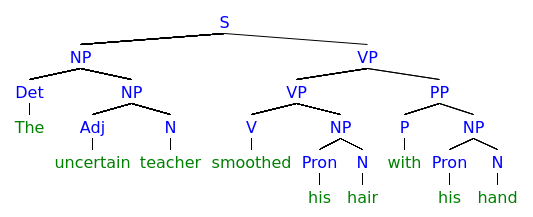
\includegraphics[width=\linewidth]{1a.png}
	\caption{\textit{The uncertain teacher smoothed his hair with his hand}
	constituency tree}
	\label{fig:1a}
\end{figure}

A confident man washed his shirt in his sink.

The strange chef served her food on his hat.

\subsection{}
\begin{align*}
	\mathrm{S} &\rightarrow \mathrm{NP~VP} \\
	\mathrm{NP} &\rightarrow \mathrm{Det~NP~|~Adj~N~|~Pron~N}\\
	\mathrm{VP} &\rightarrow \mathrm{VP~PP~|~V~NP}\\
	\mathrm{PP} &\rightarrow \mathrm{P~NP}\\
	\mathrm{Det} &\rightarrow \mathrm{the}\\
	\mathrm{Adj} &\rightarrow \mathrm{uncertain}\\
	\mathrm{N} &\rightarrow \mathrm{teacher~|~hair~|~hand}\\
	\mathrm{Pron} &\rightarrow \mathrm{his}\\
	\mathrm{V} &\rightarrow \mathrm{smoothed}\\
	\mathrm{P} &\rightarrow \mathrm{with}
\end{align*}

\section{}
\subsection{}
\begin{figure}[h!]
	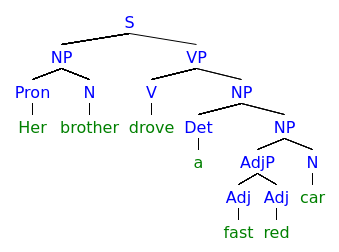
\includegraphics[width=\linewidth]{2ai.png}
	\caption{\textit{Her brother drove a fast red car} constituency tree}
	\label{fig:2ai}
\end{figure}

\begin{figure}[h!]
	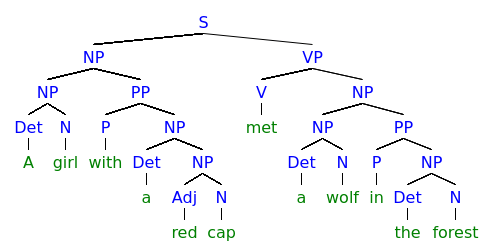
\includegraphics[width=\linewidth]{2aii.png}
	\caption{\textit{A girl with a red cap met a wolf in the forest}
	constituency tree}
	\label{fig:2aii}
\end{figure}

Labels used are S - Sentence;
NP - Noun Phrase;
VP - Verb Phrase;
Pron - Pronoun;
N - Noun;
V - Verb;
Det - Determiner;
AdjP - Adjectival Phrase;
Adj - Adjective;
P - Preposition

\subsection{}
\begin{figure}[h!]
	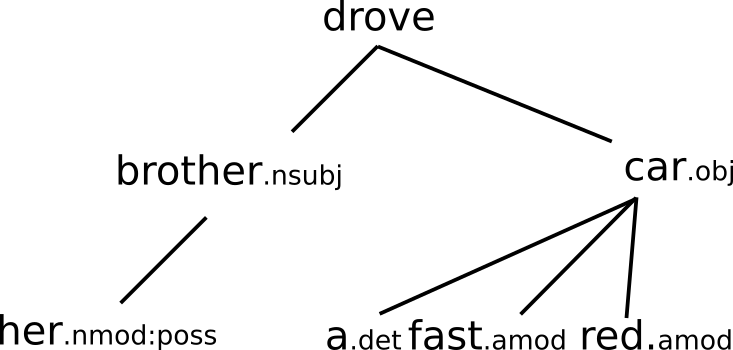
\includegraphics[width=\linewidth]{2aidep.png}
	\caption{\textit{Her brother drove a fast red car} dependency tree}
	\label{fig:2aidep}
\end{figure}

\begin{figure}[h!]
	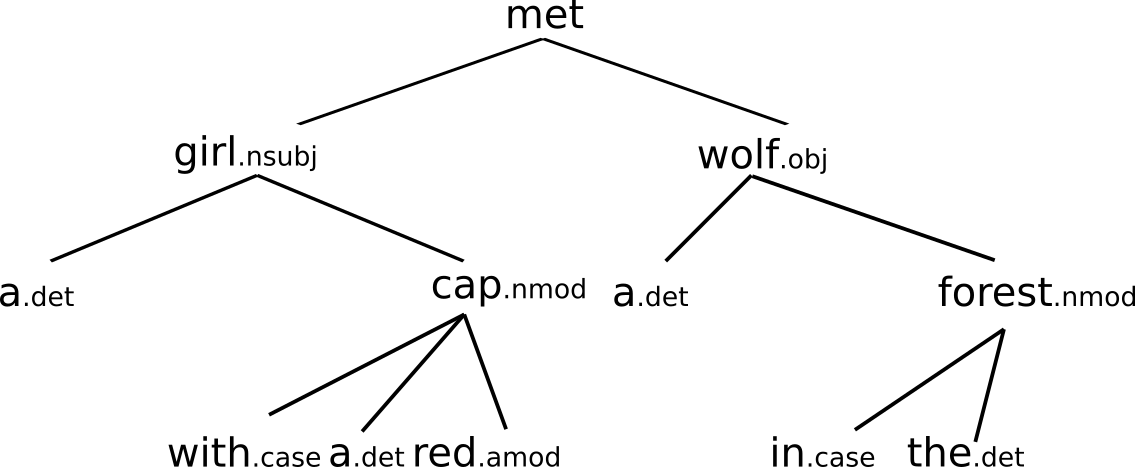
\includegraphics[width=\linewidth]{2aiidep.png}
	\caption{\textit{A girl with a red cap met a wolf in the forest} dependency
	tree}
	\label{fig:2aiidep}
\end{figure}

Syntactic functions are as used in Universal Dependencies v2.

nsubj - nominal subject;
obj - direct object;
nmod - noun as an additional argument;
nmod:poss - possessive pronoun;
det - determiner;
amod - adjectival modifier;
case - preposition;

\end{document}
